\documentclass{article}
%List of PACKAGES used
\usepackage[utf8]{inputenc}
\usepackage{graphicx}
\usepackage[dutch]{babel}
\usepackage{xcolor}
\usepackage{amsmath}
\usepackage{amssymb}
\usepackage{tabularx}
\usepackage{array}
\usepackage{hyperref}
\usepackage{multirow}
\usepackage{csquotes}
\usepackage{float}
\restylefloat{table}
\graphicspath{ {./images/} }


\title{%
  DIY Acoustic Camera \\
  \Minutes group 24 }
\author{Atom Levison, Camiel van der Marel, Sam Moerdijk, Jasper Nierse}
\date{\today}
\begin{document}

\maketitle

\newpage

\chapter{10/06/24}

\begin{table}[H]
\begin{tabular}{|p{1.5in}|p{4in}|}
\hline
Date/Time/Place &  10/06/24, 11.00-11.15/SP\\ \hline
What            &  Consultation sir Sprik\\ \hline
Who             &  AL, CM, SM, JN\\ \hline
How             &  A quick consultation what we will be doing on 10/06.  \\ \hline
What's next     &  Testing of code\\ \hline
\end{tabular}
\end{table}


\begin{table}[H]
\begin{tabular}{|p{1.5in}|p{4in}|}
\hline
Date/Time/Place & 10/06/24, 11.30-12.00/SP \\ \hline
What            &  Testing of code\\ \hline
Who             &  AL, CM, SM, JN\\ \hline
How             &  By testing the code for the acoustic camera in a room with little background noise we tried to determine if the code would work. We found that during the first few test runs the camera picked up a lot of background noise and by reducing the noise we found that the code written by CM functioned. The test setupp was determined on location and no data obtained during testing will be used further. \\ \hline
What's next     &  The code for the mics doesn't work as it should and more coding by CM and AL is needed\\ \hline
\end{tabular}
\end{table}
\begin{figure}[H]
    \centering
    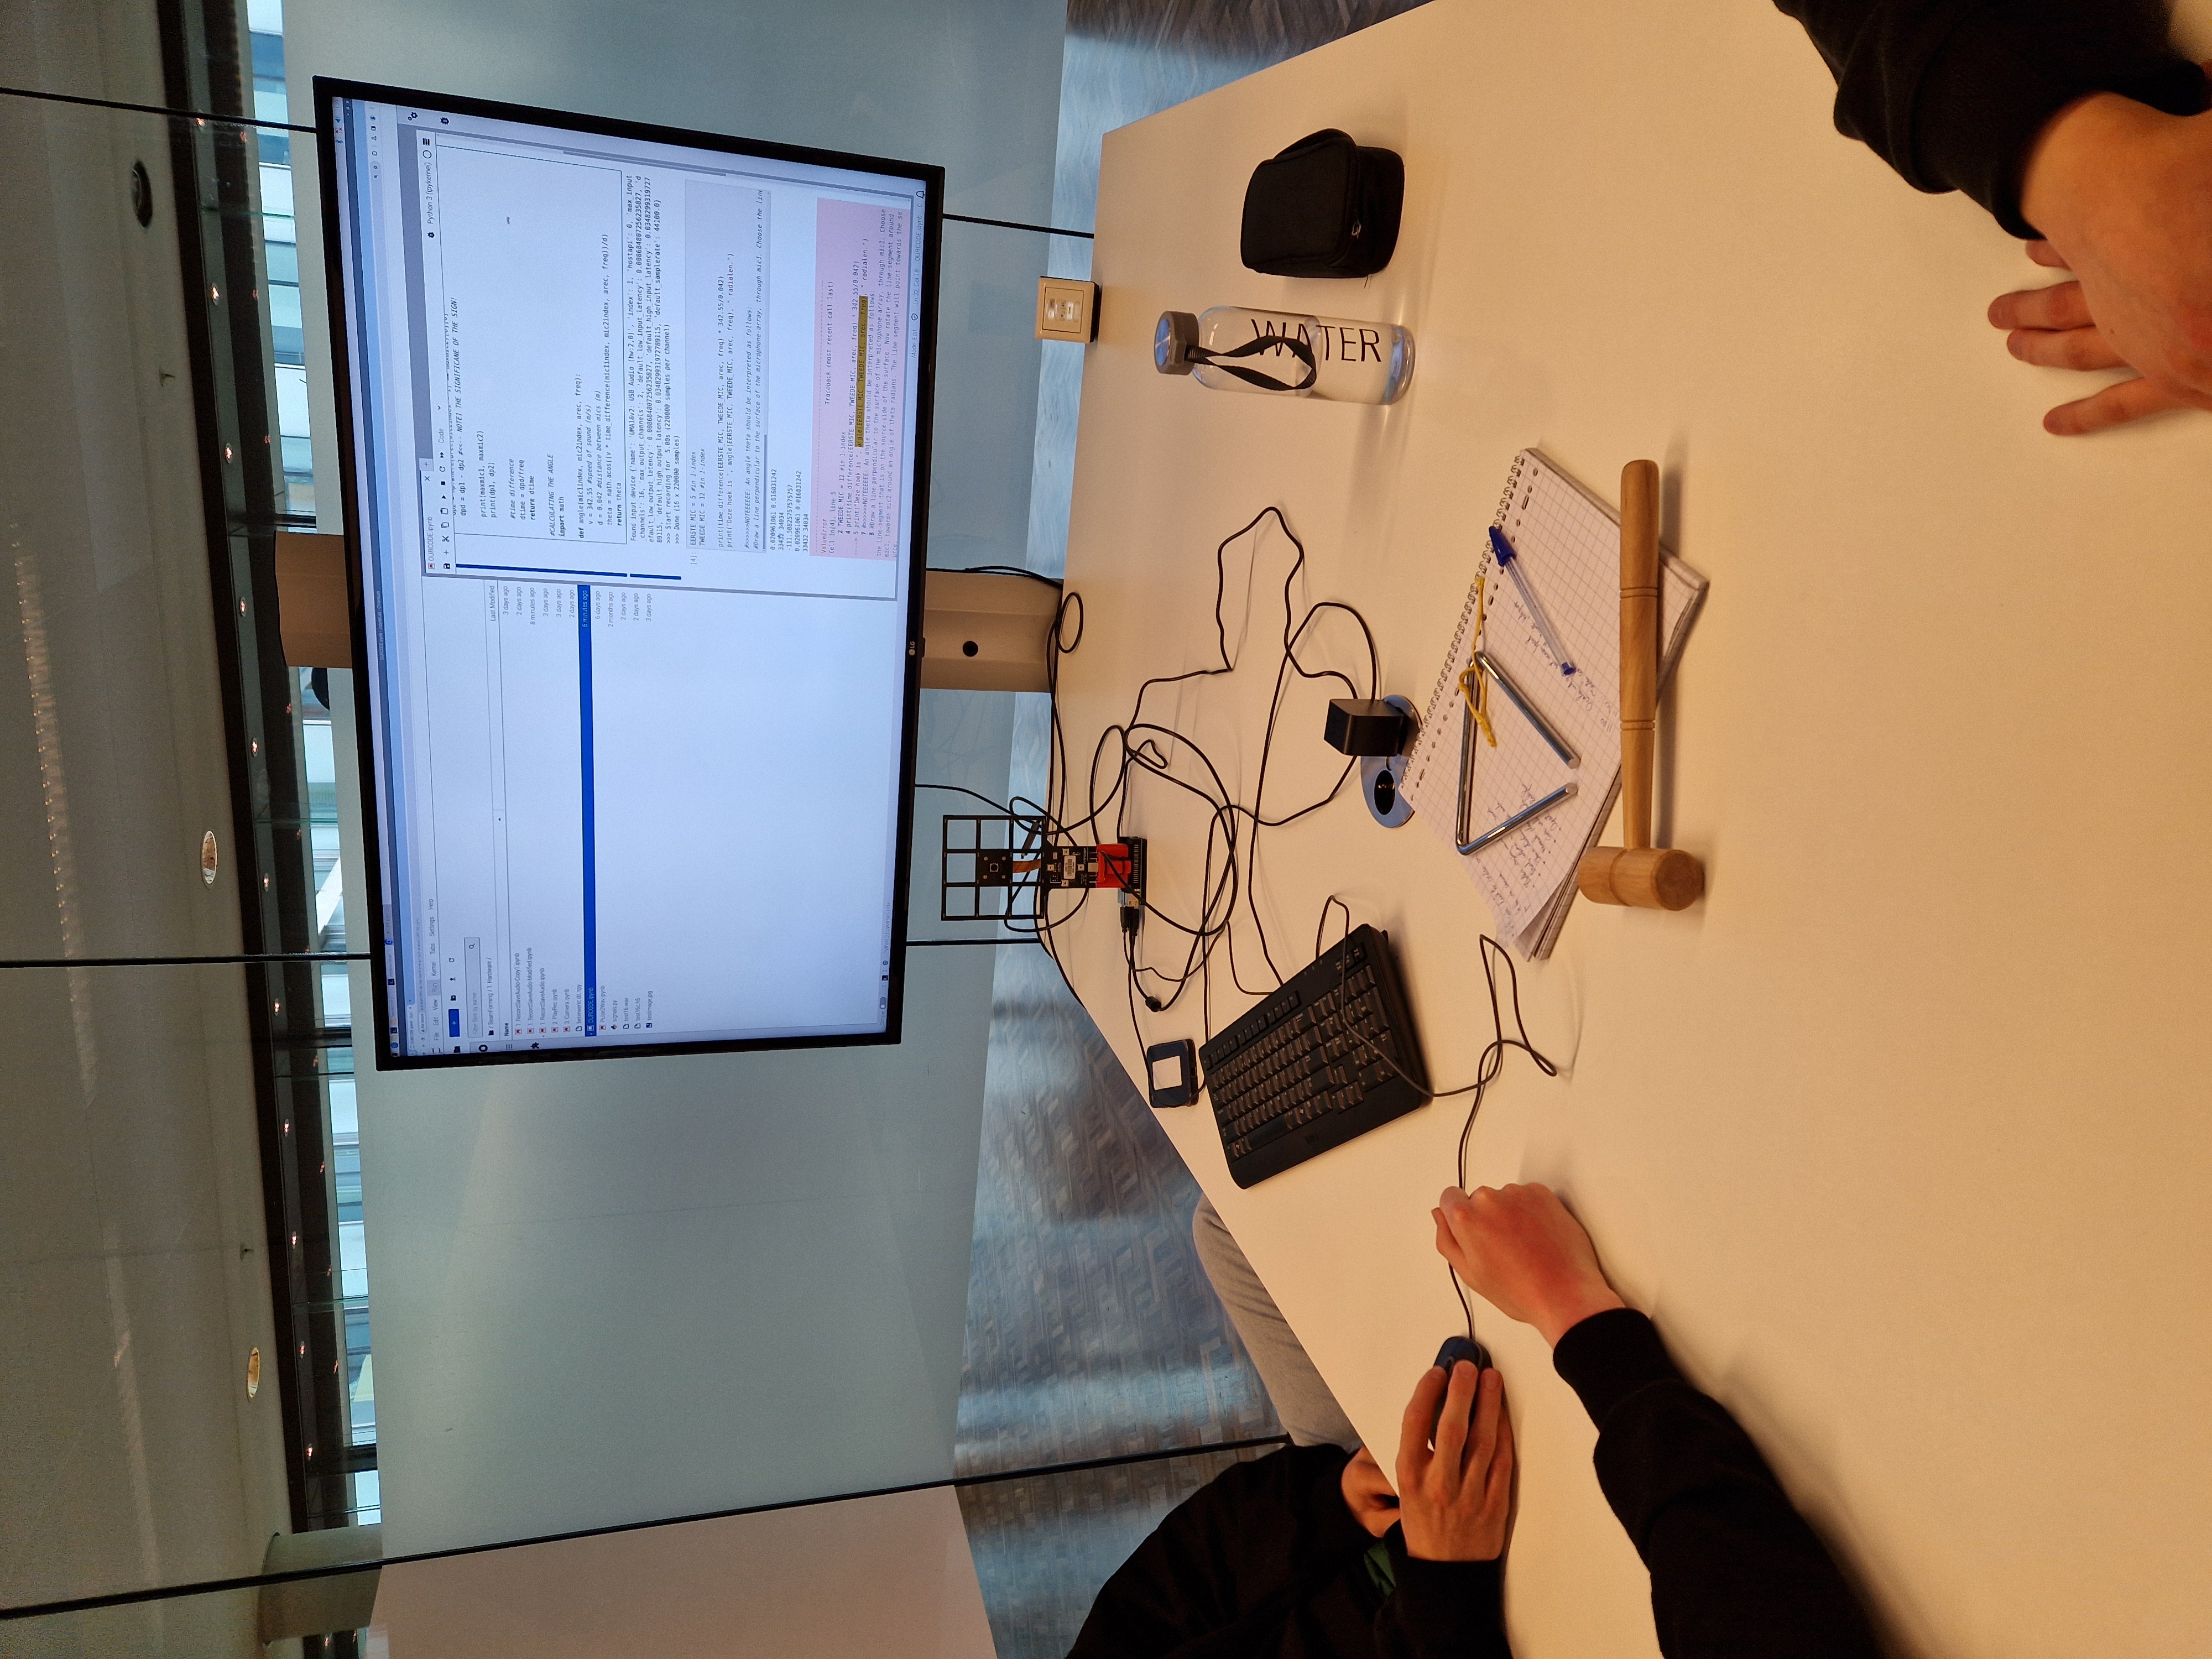
\includegraphics[width=8cm, angle =270]{20240610_113743.jpg}
    \caption{Setup during testing}   
\end{figure}

%Hier staat de foto van de opstelling.

\begin{table}[H]
\begin{tabular}{|p{1.5in}|p{4in}|}
\hline
Date/Time/Place &  10/06/24, 12.00-13.30/SP\\ \hline
What            &  Making a Minutes layout\\ \hline
Who             &  JN\\ \hline
How             &  Creating a structure for the minutes in Latex and linking this to GitHub\\ \hline
What's next     &  Making sure that everyone fills in this file so we have a complete picture of what we have done together with the GitHub Planning To Do list.\\ \hline
\end{tabular}
\end{table}

\begin{table}[H]
\begin{tabular}{|p{1.5in}|p{4in}|}
\hline
Date/Time/Place & 10/06/24, 16.30-17.30 \\ \hline
What            &  Creating a design for the poster\\ \hline
Who             &  JN \\ \hline
How             &  Completing the design for the poster in Canva\\ \hline
What's next     &  Filling in the poster with text and images after we finish the experiment.\\ \hline
\end{tabular}
\end{table}

\begin{figure}[H]
    \centering
    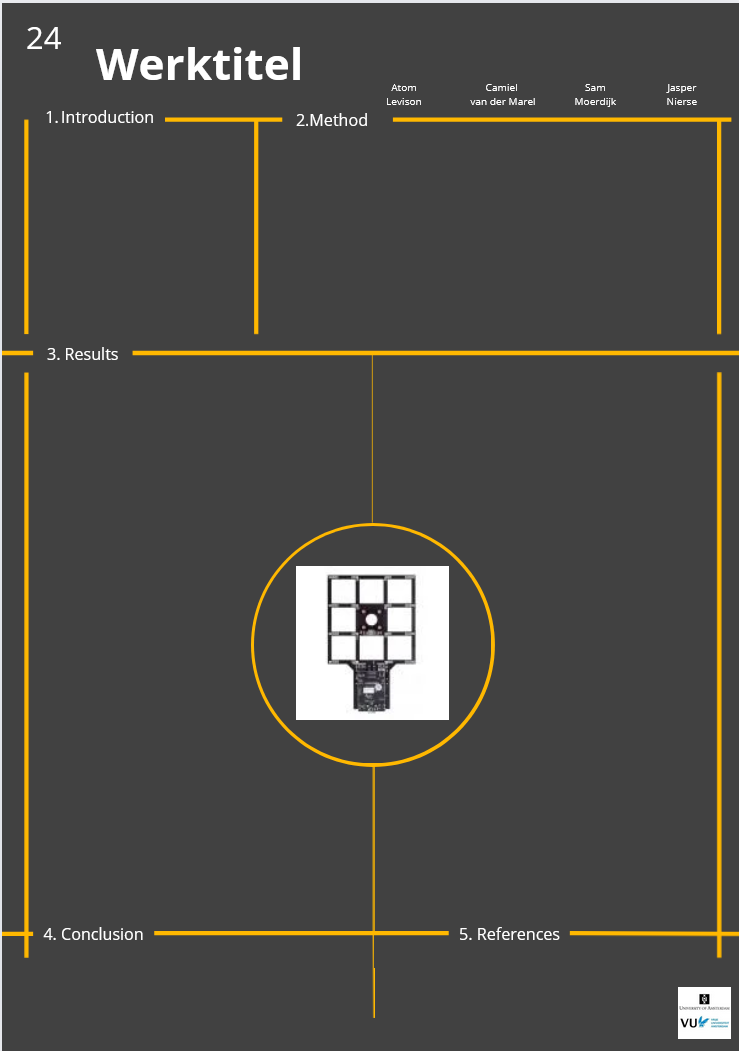
\includegraphics[width=6cm]{PosterV1.png}
    \caption{Version 1 of the empty poster with filler image.}   
\end{figure}
%Hier staat de foto van de eerste versie van de lege poster.

\begin{table}[H]
\begin{tabular}{|p{1.5in}|p{4in}|}
\hline
Date/Time/Place &  10/06/24, 12.00-13.30/SP\\ \hline
What            &  Studying literature on the triangle \\ \hline
Who             &  SM\\ \hline
How             &  With literature added to Github by Sprik, I tried to educate myself more about the triangle and its sound behavior.\\ \hline
What's next     &   Error propagation. And eventually, collect data from experiments and analyze them to understand noise behavior, and test the theories I have studied in practice.\\ \hline
\end{tabular}
\end{table}

\begin{table}[H]
\begin{tabular}{|p{1.5in}|p{4in}|}
\hline
Date/Time/Place &  10/06/24, 13.30-14.00\\ \hline
What            &  Error propagation\\ \hline
Who             &  SM\\ \hline
How             &   To calculate the error propagation, I use the partial derivatives of theta to the variables. Then I multiply the partial derivative of theta to a variable by the change in that variable and square it: $$\frac{\partial\theta}{\partial \text{variable}}\cdot\Delta\text{variable}$$ I do this for all variables and then finally take the root of the sum of these squared terms.\\ \hline
What's next     &  \\ \hline
\end{tabular}
\end{table}

\begin{table}[H]
\begin{tabular}{|p{1.5in}|p{4in}|}
\hline
Date/Time/Place &  \\ \hline
What            &  \\ \hline
Who             &  \\ \hline
How             &  \\ \hline
What's next     &  \\ \hline
\end{tabular}
\end{table}

\begin{table}[H]
\begin{tabular}{|p{1.5in}|p{4in}|}
\hline
Date/Time/Place &  \\ \hline
What            &  \\ \hline
Who             &  \\ \hline
How             &  \\ \hline
What's next     &  \\ \hline
\end{tabular}
\end{table}

\begin{table}[H]
\begin{tabular}{|p{1.5in}|p{4in}|}
\hline
Date/Time/Place &  \\ \hline
What            &  \\ \hline
Who             &  \\ \hline
How             &  \\ \hline
What's next     &  \\ \hline
\end{tabular}
\end{table}

\begin{table}[H]
\begin{tabular}{|p{1.5in}|p{4in}|}
\hline
Date/Time/Place &  \\ \hline
What            &  \\ \hline
Who             &  \\ \hline
How             &  \\ \hline
What's next     &  \\ \hline
\end{tabular}
\end{table}

\begin{table}[H]
\begin{tabular}{|p{1.5in}|p{4in}|}
\hline
Date/Time/Place &  \\ \hline
What            &  \\ \hline
Who             &  \\ \hline
How             &  \\ \hline
What's next     &  \\ \hline
\end{tabular}
\end{table}

\begin{table}[H]
\begin{tabular}{|p{1.5in}|p{4in}|}
\hline
Date/Time/Place &  \\ \hline
What            &  \\ \hline
Who             &  \\ \hline
How             &  \\ \hline
What's next     &  \\ \hline
\end{tabular}
\end{table}

\begin{table}[H]
\begin{tabular}{|p{1.5in}|p{4in}|}
\hline
Date/Time/Place &  \\ \hline
What            &  \\ \hline
Who             &  \\ \hline
How             &  \\ \hline
What's next     &  \\ \hline
\end{tabular}
\end{table}

\begin{table}[H]
\begin{tabular}{|p{1.5in}|p{4in}|}
\hline
Date/Time/Place &  \\ \hline
What            &  \\ \hline
Who             &  \\ \hline
How             &  \\ \hline
What's next     &  \\ \hline
\end{tabular}
\end{table}

\begin{table}[H]
\begin{tabular}{|p{1.5in}|p{4in}|}
\hline
Date/Time/Place &  \\ \hline
What            &  \\ \hline
Who             &  \\ \hline
How             &  \\ \hline
What's next     &  \\ \hline
\end{tabular}
\end{table}

\begin{table}[H]
\begin{tabular}{|p{1.5in}|p{4in}|}
\hline
Date/Time/Place &  \\ \hline
What            &  \\ \hline
Who             &  \\ \hline
How             &  \\ \hline
What's next     &  \\ \hline
\end{tabular}
\end{table}

\begin{table}[H]
\begin{tabular}{|p{1.5in}|p{4in}|}
\hline
Date/Time/Place &  \\ \hline
What            &  \\ \hline
Who             &  \\ \hline
How             &  \\ \hline
What's next     &  \\ \hline
\end{tabular}
\end{table}




\end{document}